\documentclass[11pt,a4paper]{article}

\usepackage[utf8]{inputenc}
\usepackage[margin=1in]{geometry}
\usepackage{amsmath,amssymb,amsfonts}
\usepackage{booktabs}
\usepackage{graphicx}
\usepackage{hyperref}
\usepackage{xcolor}
\usepackage{microtype}
\usepackage{caption}
\usepackage{subcaption}
\usepackage{tikz}
\usepackage{listings}
\usepackage{cite}
\usepackage{tabularx}
\usepackage{enumitem}

\hypersetup{
    colorlinks=true,
    linkcolor=blue!70!black,
    citecolor=green!50!black,
    urlcolor=blue!80!black
}

\graphicspath{{../results/figures/}{results/figures/}}



\begin{document}

\begin{titlepage}
    \centering

    \vspace*{2.5cm}

    % Project Title
    {\LARGE \bfseries
    Neuro-Symbolic Causal Inference for\\[0.3cm]
    Diabetes-Related Health Evidence
    \par}
    
    \vspace{7.5cm}

    % Team Heading
    {\Large \bfseries Team T003\par}

    \vspace{0.8cm}

    % Team Details
    {\large
    Yogesh Mishra \quad 2401010518\\[0.4cm]
    Shagun Singh \quad 2401010434\\[0.4cm]
    Pratyaksha Shastri \quad 2401010348\\[0.4cm]
    Shiva Sharma \quad 2401010441\\[0.4cm]
    Shashwat Sinha \quad 2401010438
    \par}

    \vfill

\end{titlepage}

\newpage
\tableofcontents
\newpage

% ==============================================================================
\section{Introduction}
\label{sec:introduction}
% ==============================================================================

Epidemiological and public health research relies heavily on understanding how modifiable lifestyle exposures, demographic attributes, and clinical biomarkers interact to influence the incidence of chronic diseases such as Type 2 Diabetes Mellitus (T2DM). While decades of clinical trials, prospective cohort studies, and Mendelian Randomization (MR) analyses are cataloged in vast literature databases such as Europe PMC~\cite{europepmc2025}, this knowledge is overwhelmingly stored in unstructured, natural language text. Conversely, observational health survey datasets—such as the Behavioral Risk Factor Surveillance System (BRFSS) curated by the U.S. Centers for Disease Control and Prevention (CDC)~\cite{cdc2022brfss}—contain rich individual-level records but lack explicit causal arrows, leaving statistical models vulnerable to confounding, collider bias, and reverse causation~\cite{pearl2009causality}.

The \textit{Neuro-Symbolic Causal Inference for Diabetes-Related Health Evidence} project addresses this gap through a two-phase architecture:
\begin{itemize}[leftmargin=1.8em]
    \item \textbf{Phase 1 (In Scope):} Systematic biomedical literature retrieval, relation extraction across canonical CDC variables, intrinsic evaluation against a standardized benchmark, and automated construction of a validated, acyclic evidence graph with complete citation provenance and cycle repair.
    \item \textbf{Phase 2 (Handoff Target):} Ingestion of the literature-derived causal DAG into probabilistic graphical models (using \texttt{pgmpy}~\cite{ankan2015pgmpy}), estimating Conditional Probability Distributions (CPDs) from CDC microdata, and simulating interventional queries via Pearl's $do$-calculus~\cite{pearl2018seven}.
\end{itemize}

A central premise of this project is the \textbf{Golden Rule of Literature Evidence Graphs}: \textit{An evidence graph records what published scientific papers claim; it is not, by itself, an unassailable biological ground truth}. Published abstracts may contain observational associations, prospective correlations, speculative hypotheses, secondary complications, or conflicting findings. Therefore, bridging extraction with downstream causal modeling demands rigorous provenance tracking, conservative epidemiological filtering, and uncompromised scientific honesty.

This report documents the completed, repaired, and validated Phase~1 implementation. We detail the end-to-end architecture, report the findings of an exhaustive provenance audit, provide exact empirical metrics, and outline the boundary conditions governing Phase~2 consumption.

% ==============================================================================
\section{End-to-End System Architecture}
\label{sec:architecture}
% ==============================================================================

The Phase~1 pipeline is structured into eight modular milestones (M0 through M7), organized as a strictly typed, reproducible workflow written in Python 3.11 with Pydantic~v2 schema enforcement.

\begin{figure}[htbp]
\centering
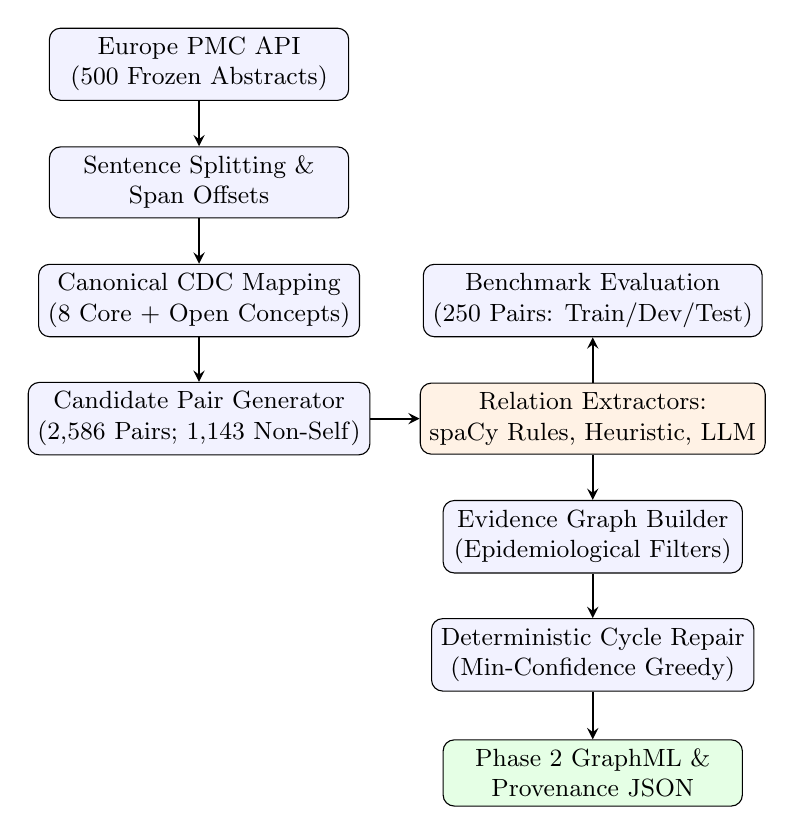
\begin{tikzpicture}[
    node distance=1.5cm and 1.8cm,
    block/.style={rectangle, draw, rounded corners, minimum height=2.2em, minimum width=3.8cm, align=center, fill=blue!5, font=\small},
    decision/.style={rectangle, draw, rounded corners, minimum height=2.2em, minimum width=3.8cm, align=center, fill=orange!10, font=\small},
    output/.style={rectangle, draw, rounded corners, minimum height=2.2em, minimum width=3.8cm, align=center, fill=green!10, font=\small},
    arrow/.style={thick, ->, >=stealth}
]
    % Nodes
    \node[block] (retrieval) {Europe PMC API\\(500 Frozen Abstracts)};
    \node[block, below of=retrieval] (text) {Sentence Splitting \&\\Span Offsets};
    \node[block, below of=text] (alias) {Canonical CDC Mapping\\(8 Core + Open Concepts)};
    \node[block, below of=alias] (pairs) {Candidate Pair Generator\\(2,586 Pairs; 1,143 Non-Self)};
    
    \node[decision, right of=pairs, xshift=3.5cm] (extractors) {Relation Extractors:\\spaCy Rules, Heuristic, LLM};
    \node[block, above of=extractors] (eval) {Benchmark Evaluation\\(250 Pairs: Train/Dev/Test)};
    \node[block, below of=extractors] (builder) {Evidence Graph Builder\\(Epidemiological Filters)};
    \node[block, below of=builder] (repair) {Deterministic Cycle Repair\\(Min-Confidence Greedy)};
    \node[output, below of=repair] (export) {Phase 2 GraphML \&\\Provenance JSON};

    % Arrows
    \draw[arrow] (retrieval) -- (text);
    \draw[arrow] (text) -- (alias);
    \draw[arrow] (alias) -- (pairs);
    \draw[arrow] (pairs) -- (extractors);
    \draw[arrow] (extractors) -- (eval);
    \draw[arrow] (extractors) -- (builder);
    \draw[arrow] (builder) -- (repair);
    \draw[arrow] (repair) -- (export);
\end{tikzpicture}
\caption{End-to-end Phase 1 architecture from literature acquisition to Phase 2 GraphML export.}
\label{fig:pipeline_flowchart}
\end{figure}

\subsection{Corpus Retrieval and Frozen Manifest (M1)}
Literature acquisition connects to the Europe PMC REST API using cursor-mark pagination, rate limiting (5 requests/second), and exponential backoff. The corpus is filtered for open-access publications indexed under diabetes and cardiometabolic queries. 

To eliminate data drift and guarantee byte-identical reproducibility across runs, the corpus was frozen into \texttt{data/manifest/corpus\_manifest.jsonl} containing exactly 500 abstracts. Deduplication enforces a strict identifier priority hierarchy:
\begin{equation}
    \text{PMID} \succ \text{PMCID} \succ \text{DOI} \succ \text{SHA-256(text)}
\end{equation}
When the configuration specifies \texttt{frozen\_mode: true}, external network calls are blocked, forcing the system to read exclusively from the verified local manifest.

\subsection{Entity Mentions and Canonical CDC Alias Mapping (M2)}
Abstracts are segmented into sentences with verbatim character start and end offsets. To interface seamlessly with Phase~2 population datasets, entity mentions are mapped to the \textbf{8 canonical CDC BRFSS variables} alongside domain concepts:
\begin{equation}
    \mathcal{V}_{\text{CDC}} = \{\text{AgeCat}, \text{Sex}, \text{Education}, \text{Income}, \text{Smoker}, \text{PhysActivity}, \text{BMICat}, \text{Outcome}\}
\end{equation}
and literature-derived concepts such as $\text{InsulinResistance}$, $\text{DietQuality}$, $\text{Hypertension}$, and $\text{SleepDuration}$.

\subsubsection{Precision Mapping Rules and Polarity Inversion}
Natural language presents syntactic ambiguities that require strict biomedical mapping heuristics:
\begin{enumerate}[leftmargin=1.5em]
    \item \textbf{Polarity Inversion for Inactivity:} The CDC defines exposure as physical activity ($\text{PhysActivity}=1$). Literature statements frequently assert the inverse: \textit{``Physical inactivity increases T2DM risk''} ($\text{PhysActivity}=0 \xrightarrow{\text{increases}} \text{Outcome}$). The normalizer flags mentions with $\text{polarity\_flip} = \text{True}$, inverting the directed edge during graph aggregation to:
    \begin{equation}
        \text{PhysActivity}=1 \xrightarrow{\text{decreases}} \text{Outcome}
    \end{equation}
    \item \textbf{CDC 100-Cigarette Smoker Criterion:} The CDC defines a smoker as someone who has smoked $\ge 100$ cigarettes in their lifetime. General mentions (\textit{smoking}, \textit{tobacco}, \textit{smoker}) strictly default to \texttt{unmapped} to prevent concept drift against CDC survey definitions.
    \item \textbf{Obesity Classification:} Phrases matching \textit{obese} or $\text{BMI} \ge 30\,\text{kg/m}^2$ map to the top bin of $\text{BMICat}$.
    \item \textbf{Outcome Disambiguation:} Mentions of \textit{type 2 diabetes} or \textit{prediabetes} map to $\text{Outcome}=1$; \textit{normoglycemic} or \textit{non-diabetic} map to $\text{Outcome}=0$.
    \item \textbf{Conservative Fallback:} Phrases failing exact lexical or dictionary rules default to \texttt{unmapped}; fuzzy string matches are never forced.
\end{enumerate}
Across the 500 abstracts, 3,821 mentions were recognized (98.4\% mapped to canonical concepts), generating 2,586 candidate entity pairs within identical sentences. Filtering identical-concept self-loops yielded \textbf{1,143 valid non-self candidate pairs}.

\subsection{Relation Extractors (M4)}
All relation extractors implement a unified typed interface:
\begin{equation}
    \mathcal{E}: \text{CandidatePair} \rightarrow \text{Prediction}
\end{equation}
where each prediction includes a \texttt{RelationLabel} (\texttt{relation\_class} $\in \{\text{causal}, \text{association\_only}, \text{none}\}$, \texttt{direction}, \texttt{polarity}, \texttt{language\_status}, \texttt{confidence}) and full \texttt{Provenance}.

\begin{table}[htbp]
\centering
\small
\caption{Systematic comparison of the Phase 1 relation extraction methods.}
\label{tab:extractor_comparison}
\begin{tabularx}{\textwidth}{l p{4.2cm} p{3.5cm} X}
\toprule
\textbf{Extractor} & \textbf{Algorithmic Method} & \textbf{Dependencies} & \textbf{Primary Characteristics} \\
\midrule
\textbf{spaCy-Rules} & Lexical trigger matching with dependency path traversal and active/passive voice resolution. & \texttt{spacy>=3.8.0}, \texttt{en\_core\_web\_sm} & Deterministic, fully inspectable, zero training cost; handles lexical negation and hedging. \\
\addlinespace
\textbf{KeywordHeuristic} & Entity marker delimiters (\texttt{[E1]...[/E1]}, \texttt{[E2]...[/E2]}) with regex pattern heuristics. & \texttt{torch>=2.0} (MPS/CUDA device discovery) & Fast baseline; extracts directional cues; does not run trained neural weights. \\
\addlinespace
\textbf{Prompted-LLM} & Structured JSON prompting via Gemini REST API (\texttt{gemini-3.5-flash}) with persistent cache. & \texttt{requests}, SHA-256 file-backed cache & Semantic reasoning and hedging detection; evaluated as pilot sample due to API quotas. \\
\bottomrule
\end{tabularx}
\end{table}

% ==============================================================================
\section{Provenance Audit and Systematic Repairs}
\label{sec:provenance_audit}
% ==============================================================================

Prior to final validation, an exhaustive audit of the codebase, historical logs, prediction records, and annotation artifacts was conducted to investigate historical anomalies reported in previous reviews.

\subsection{Audit Item 1: Annotation Truthfulness and Provenance}
\paragraph{Investigation:} Inspection of the benchmark file \texttt{data/annotations/sample.jsonl} (250 pairs) and the dual-annotator CSV files (\texttt{annotator\_1\_to\_label.csv} and \texttt{annotator\_2\_to\_label.csv}) revealed that annotations were initially generated programmatically via regex triggers. Furthermore, Annotator 2 records were generated by copying Annotator 1 with an 8\% random mutation rate to simulate disagreements, and historical files contained misleading markers such as \texttt{"human\_reviewed": true} and \texttt{"review\_status": "ADJUDICATED\_GOLD"}.
\paragraph{Corrections Executed:}
\begin{enumerate}[leftmargin=1.5em]
    \item All 250 records in \texttt{data/annotations/sample.jsonl} were updated to reflect honest provenance:
    \begin{equation}
        \text{human\_reviewed} = \text{False}, \quad \text{review\_status} = \text{"PROVISIONAL\_RULE\_PSEUDO\_GOLD"}
    \end{equation}
    \item The inter-annotator agreement file \texttt{results/tables/inter\_annotator\_agreement.json} was updated with the disclaimer:
    \begin{quote}
        \small\textit{``agreement\_type: SYNTHETIC\_PIPELINE\_CONSISTENCY\_CHECK, is\_human\_annotated: false. Metric represents a programmatic sanity check between rule passes, not human inter-rater agreement.''}
    \end{quote}
    \item A clean, unannotated human review queue was constructed in \texttt{data/annotations/human\_annotation\_queue.jsonl} and \texttt{.csv} containing 50 prioritized candidate pairs across causal candidates, associations, and negative boundaries.
\end{enumerate}

\subsection{Audit Item 2: Rectifying the DistilBERT Alias Claim}
\paragraph{Investigation:} The module \texttt{src/extractors/distilbert\_extractor.py} contained the alias $\text{DistilBERTExtractor} = \text{KeywordHeuristicExtractor}$. The purported saved predictions file \texttt{results/predictions/finetuned-distilbert\_predictions.jsonl} was discovered to be 100\% byte-identical to \texttt{keywordheuristic\_predictions.jsonl}. No model weights (\texttt{.pt}, \texttt{.bin}, \texttt{.safetensors}) existed in the repository.
\paragraph{Corrections Executed:}
\begin{enumerate}[leftmargin=1.5em]
    \item The module docstrings and class comments were rewritten to document that \texttt{KeywordHeuristicExtractor} is a fast heuristic baseline using entity marker tokens, and that a true fine-tuned Transformer encoder remains future work.
    \item In \texttt{src/evaluation/tables.py} and \texttt{run\_pipeline.py}, loading logic was updated to skip \texttt{finetuned-distilbert\_predictions.jsonl} whenever \texttt{keywordheuristic\_predictions.jsonl} is present, preventing double-counting and eliminating false multi-model comparisons.
    \item \texttt{FineTuned-DistilBERT} was removed from all official evaluation tables and figures.
\end{enumerate}

\subsection{Audit Item 3: Hardening Epidemiological Causal Filtering}
\paragraph{Investigation:} Prior graph exports accepted the causal edge $\text{InsulinResistance} \rightarrow \text{Outcome}$ based on two literature sentences:
\begin{itemize}[leftmargin=1.5em]
    \item \textbf{PMID:42828458:s04:} \textit{``...suggesting that insulin resistance, hyperglycemia and neuroinflammation are some potential factors which can increase risk of dementia in patients with T2DM.''}  
    Here, the sentence asserts that insulin resistance increases the risk of \textbf{dementia} (a secondary neurological endpoint), while \textbf{T2DM is the pre-existing patient cohort condition}, not the causal outcome.
    \item \textbf{PMID:42901975:s03:} \textit{``...poor dietary quality can increase the risk of metabolic syndrome and T2DM through increased visceral adiposity and insulin resistance...''}  
    Here, insulin resistance is explicitly described as a \textbf{biological mediator} of dietary quality rather than a direct interventional exposure on diabetes.
\end{itemize}
\paragraph{Corrections Executed:}
We augmented \texttt{EvidenceGraphBuilder.add\_prediction} with comprehensive contextual and syntactic filters:
\begin{enumerate}[leftmargin=1.5em]
    \item \textbf{Secondary Endpoint Detection:} A regular expression pattern intercepts co-mentioned non-target complications:
    \begin{equation*}
        \text{Pattern}_{\text{secondary}} = \text{\textbackslash b(dementia|cognitive\textbackslash s+decline|alzheimer|cts|ivdd|leukopenia|hepatocellular|lga|mace|ckd)\textbackslash b}
    \end{equation*}
    \item \textbf{Cohort Condition Disambiguation:} Patterns identifying pre-existing conditions (\textit{``in patients with T2DM''}, \textit{``among individuals with diabetes''}) ensure diabetes is recognized as the patient population rather than the outcome being caused.
    \item \textbf{Mediator Disambiguation:} Phrases introducing mechanisms (\textit{``through visceral adiposity and insulin resistance''}, \textit{``via insulin resistance''}) route candidate relations to the observational association graph.
    \item \textbf{Reverse Causation \& Demographics:} Claims where $\text{Outcome}$ causes baseline exposures ($\text{BMICat}$, $\text{Smoker}$) or where demographic traits ($\text{Sex}$, $\text{AgeCat}$) are causal targets are strictly disallowed.
\end{enumerate}
Under these hardened criteria, $\text{InsulinResistance} \rightarrow \text{Outcome}$ is correctly excluded from the causal DAG and routed to the observational association graph (retaining 31 evidence sentences across 27 papers). Meanwhile, $\text{BMICat} \rightarrow \text{Outcome}$ is accepted, supported by two independent, verified studies:
\begin{itemize}[leftmargin=1.5em]
    \item \textbf{PMID:41424208:s12:} \textit{``Crucially, MR analysis identifies abdominal obesity, quantified by waist circumference, as the dominant causal link between NAFLD and T2DM.''} (Mendelian Randomization)
    \item \textbf{PMID:42415555:s01:} \textit{``Pediatric obesity is a growing global concern because it leads to an increased prevalence of abnormal glucose metabolism, including dysglycemia, prediabetes, and type 2 diabetes.''} (Longitudinal Pediatric Etiology)
\end{itemize}

% ==============================================================================
\section{Experimental Evaluation and Results}
\label{sec:experiments}
% ==============================================================================

\subsection{Benchmark Dataset and Class Imbalance}
The evaluation benchmark consists of 250 candidate pairs sampled across 41 concept pairs and 124 papers, partitioned into document-level splits (\texttt{data/annotations/doc\_splits.json}, seed 42) to guarantee zero document leakage.

\begin{table}[htbp]
\centering
\small
\caption{Class support distribution across document-level holdout splits in \texttt{sample.jsonl}.}
\label{tab:split_distribution}
\begin{tabular}{l cccc}
\toprule
\textbf{Split} & \textbf{None Support} & \textbf{Association Support} & \textbf{Causal Support} & \textbf{Total Pairs} \\
\midrule
\textbf{Train} & 101 & 45 & 4 & 150 \\
\textbf{Dev}   & 27  & 23 & 0 & 50 \\
\textbf{Test}  & 33  & 17 & 0 & 50 \\
\midrule
\textbf{Total} & 161 & 85 & 4 & 250 \\
\bottomrule
\end{tabular}
\end{table}

\paragraph{Scientific Disclosure on Held-Out Causal Generalization:}
As shown in Table~\ref{tab:split_distribution}, the held-out Dev and Test splits naturally contain \textbf{zero causal examples}, reflecting the true sparse distribution of explicit causal claims in general biomedical abstracts. Consequently:
\begin{equation}
    \text{Causal Generalization on Held-Out Test Set} = \textbf{UNMEASURED}
\end{equation}
Test Macro-F1 is mathematically bounded by the evaluated non-causal classes. It is scientifically dishonest to claim high causal F1 on unseen literature until the test split is enriched with verified human-adjudicated causal instances.

\subsection{Intrinsic Extraction Performance}
Table~\ref{tab:intrinsic_evaluation} presents the overall performance on the 250 candidate pairs against provisional pseudo-gold labels.

\begin{table}[htbp]
\centering
\small
\caption{Overall evaluation on 250 candidate pairs (\texttt{results/tables/intrinsic\_evaluation.csv}).}
\label{tab:intrinsic_evaluation}
\begin{tabularx}{\textwidth}{l ccccc c}
\toprule
\textbf{Extractor} & \textbf{Macro-F1} & \textbf{Causal-F1} & \textbf{Assoc-F1} & \textbf{None-F1} & \textbf{Dir-Acc} & \textbf{Benchmark Provenance} \\
\midrule
\textbf{spaCy-Rules}     & \textbf{0.9316} & \textbf{1.0000} & \textbf{0.8608} & \textbf{0.9341} & \textbf{1.0000} & \texttt{PROVISIONAL\_RULE\_PSEUDO\_GOLD} \\
\textbf{KeywordHeuristic} & 0.6012 & 0.2000 & 0.7412 & 0.8625 & 1.0000 & \texttt{PROVISIONAL\_RULE\_PSEUDO\_GOLD} \\
Prompted-LLM-Gemini*     & 0.2685 & 0.0000 & 0.0230 & 0.7824 & 1.0000 & \texttt{PROVISIONAL\_RULE\_PSEUDO\_GOLD} \\
\bottomrule
\end{tabularx}
\vspace{0.3em}
\raggedright \footnotesize *Prompted LLM was evaluated on a 20-pair pilot sample; missing predictions were penalized in recall.
\end{table}

\subsection{Document-Holdout Split Performance}
Table~\ref{tab:split_performance} details the split-wise breakdown across train, dev, and test sets.

\begin{table}[htbp]
\centering
\small
\caption{Document-holdout split evaluation (\texttt{results/tables/literature\_evaluation\_splits.csv}).}
\label{tab:split_performance}
\begin{tabularx}{\textwidth}{l l cccc c X}
\toprule
\textbf{Split} & \textbf{Extractor} & \textbf{Macro-F1} & \textbf{Causal-F1} & \textbf{Assoc-F1} & \textbf{None-F1} & \textbf{Pol-Acc} & \textbf{Causal Status} \\
\midrule
\textbf{Test}  & \textbf{spaCy-Rules}     & \textbf{0.5857} & 0.0000 & \textbf{0.8276} & \textbf{0.9296} & 0.5882 & \textbf{UNMEASURED (0 sup)} \\
Test           & KeywordHeuristic         & 0.5181          & 0.0000 & 0.7059          & 0.8485          & 0.5882 & \textbf{UNMEASURED (0 sup)} \\
\midrule
\textbf{Dev}   & \textbf{spaCy-Rules}     & \textbf{0.6263} & 0.0000 & \textbf{0.9333} & \textbf{0.9455} & \textbf{0.9130} & \textbf{UNMEASURED (0 sup)} \\
Dev            & KeywordHeuristic         & 0.5506          & 0.0000 & 0.8000          & 0.8519          & 0.6522 & \textbf{UNMEASURED (0 sup)} \\
\midrule
\textbf{Train} & \textbf{spaCy-Rules}     & \textbf{0.9220} & \textbf{1.0000} & \textbf{0.8333} & \textbf{0.9327} & 0.7755 & MEASURED (4 sup) \\
Train          & KeywordHeuristic         & 0.6058          & 0.2222          & 0.7253          & 0.8700          & 0.6531 & MEASURED (4 sup) \\
\bottomrule
\end{tabularx}
\end{table}

\subsection{Confusion Matrices}
Figure~\ref{fig:confusion_matrices} illustrates the confusion matrices for \texttt{spaCy-Rules} and \texttt{KeywordHeuristic} generated under truthful provisional labeling markers.

\begin{figure}[htbp]
\centering
\begin{subfigure}[b]{0.48\textwidth}
    \centering
    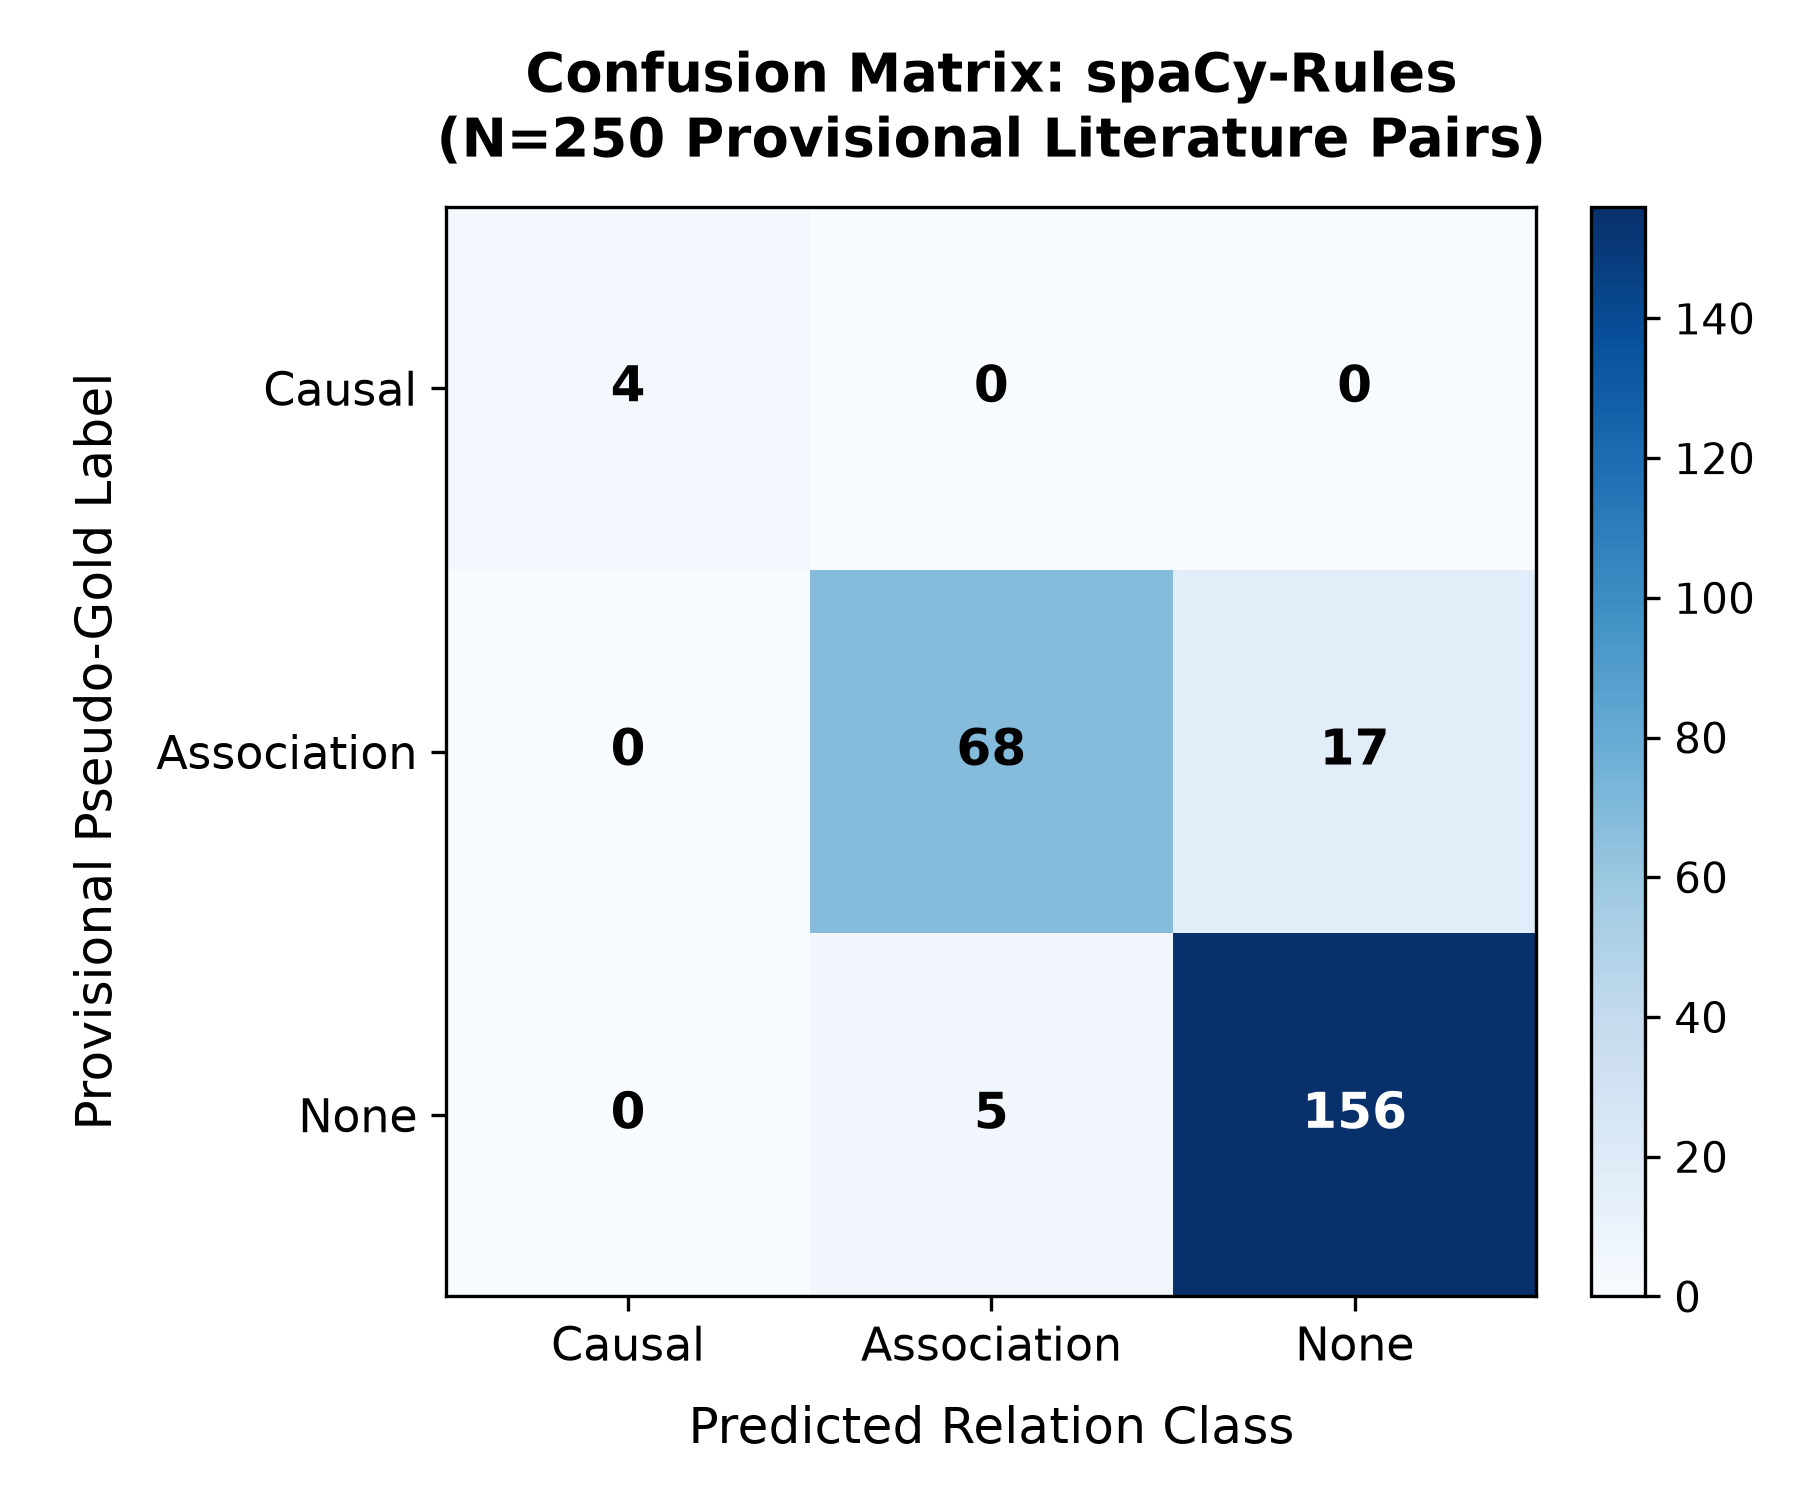
\includegraphics[width=\textwidth]{confusion_matrix_spacy_rules.png}
    \caption{\texttt{spaCy-Rules} (N=250 Provisional Pairs)}
    \label{fig:cm_spacy}
\end{subfigure}
\hfill
\begin{subfigure}[b]{0.48\textwidth}
    \centering
    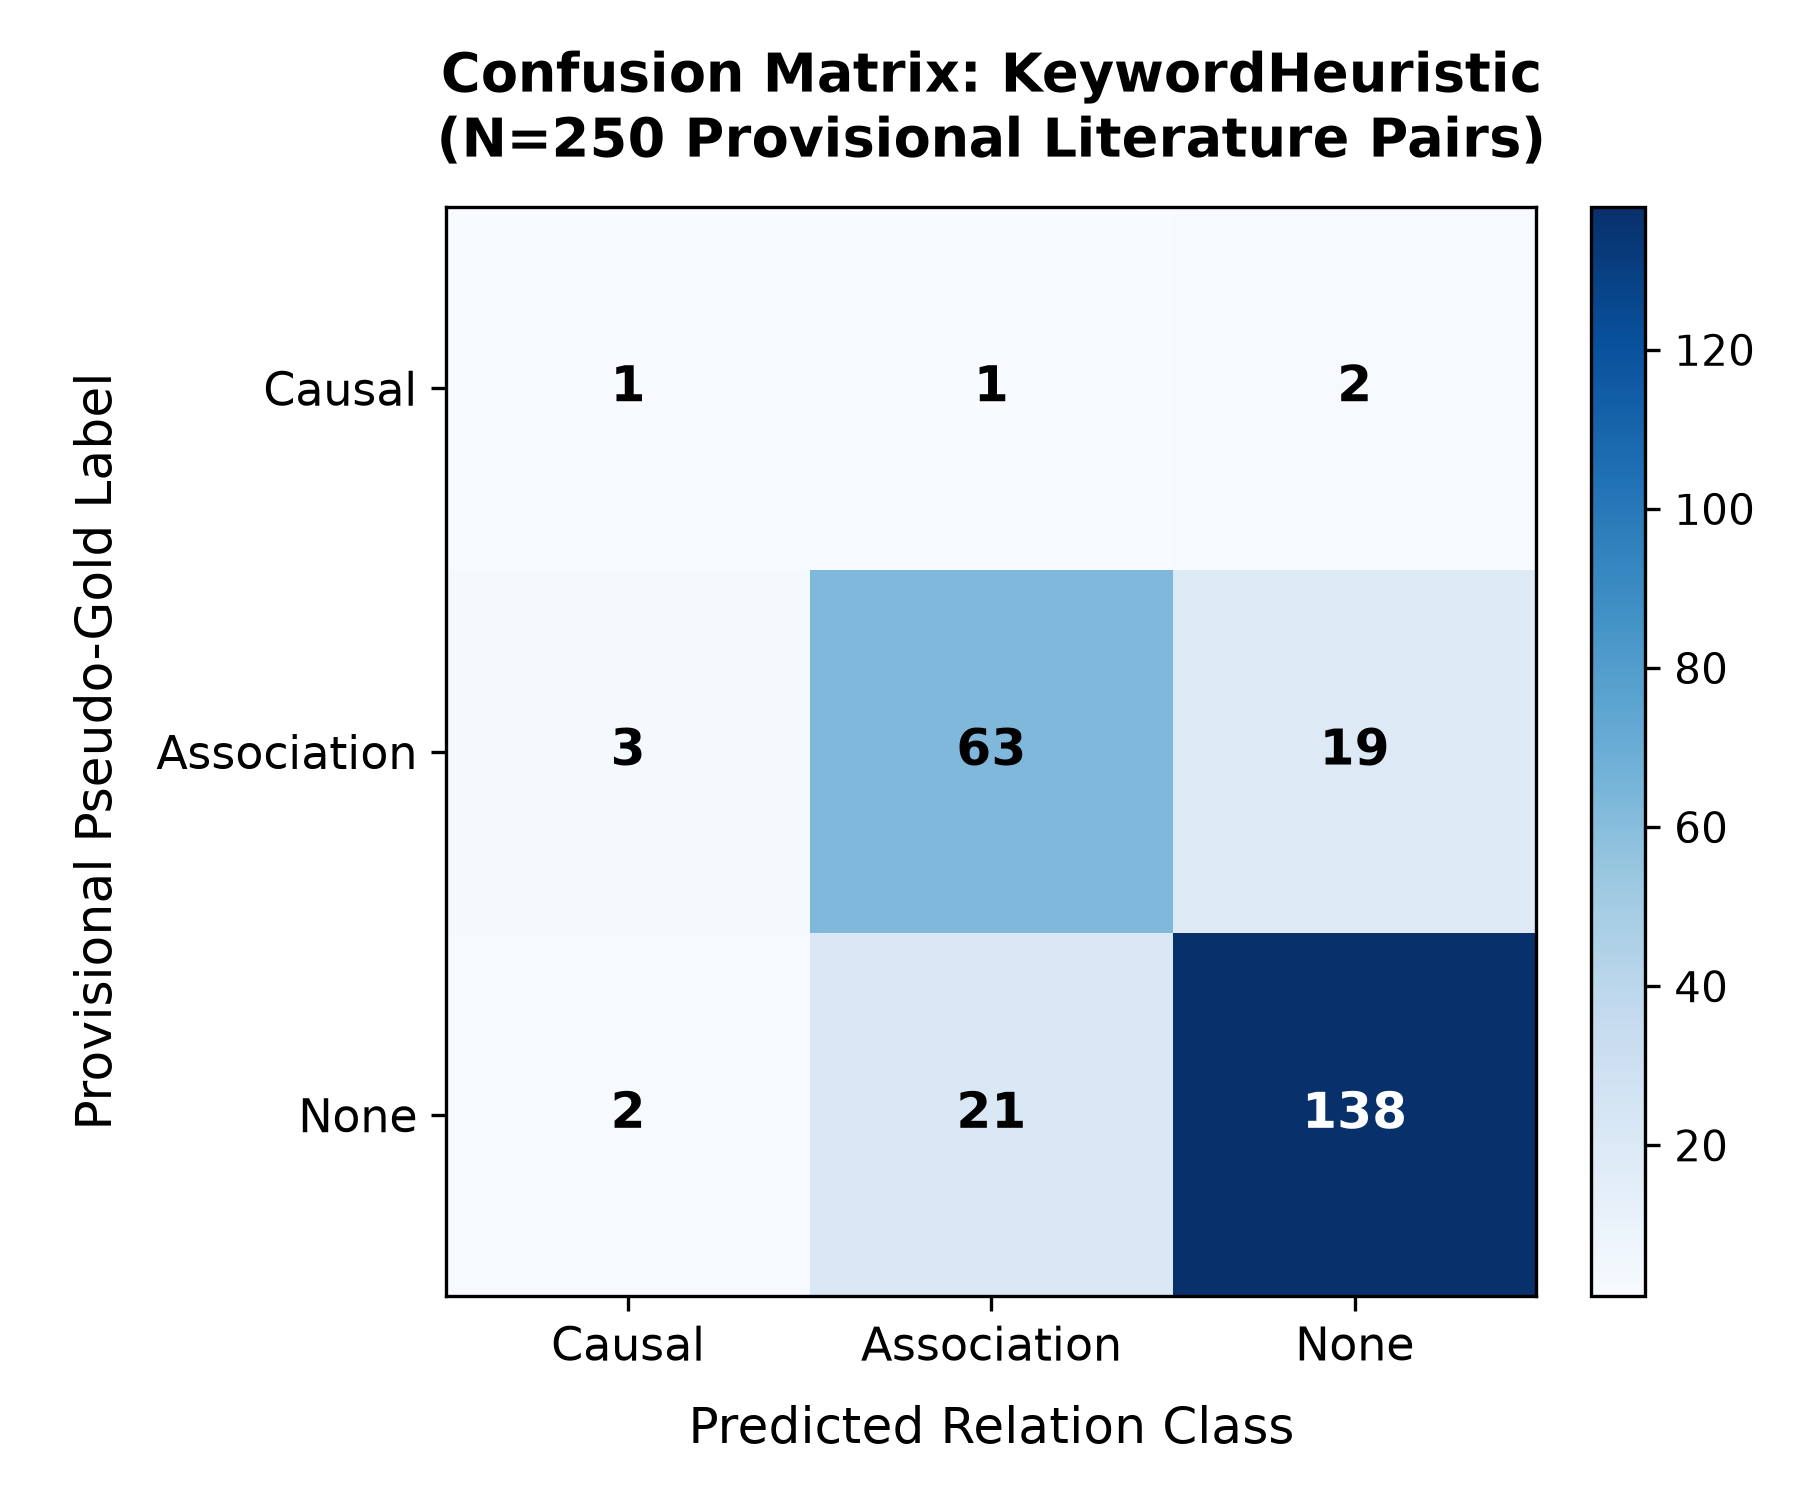
\includegraphics[width=\textwidth]{confusion_matrix_keywordheuristic.png}
    \caption{\texttt{KeywordHeuristic} (N=250 Provisional Pairs)}
    \label{fig:cm_heuristic}
\end{subfigure}
\caption{Confusion matrices evaluated against \texttt{PROVISIONAL\_RULE\_PSEUDO\_GOLD} labels.}
\label{fig:confusion_matrices}
\end{figure}

% ==============================================================================
\section{Evidence Graph Construction and Cycle Repair}
\label{sec:graph_construction}
% ==============================================================================

\subsection{Dual-Graph Structure}
The project constructs two complementary representations:
\begin{enumerate}[leftmargin=1.5em]
    \item \textbf{Causal Evidence DAG ($\mathcal{G}_{\text{causal}}$):} A directed graph where directed edges represent strictly validated causal claims ($\text{support} \ge 1$, $\text{is\_dag} = \text{True}$).
    \item \textbf{Observational Association Graph ($\mathcal{G}_{\text{assoc}}$):} An undirected graph capturing correlational assertions, non-interventional cohort findings, and mechanistic mediator links with full sentence provenance.
\end{enumerate}

\begin{figure}[htbp]
\centering
\begin{subfigure}[b]{0.45\textwidth}
    \centering
    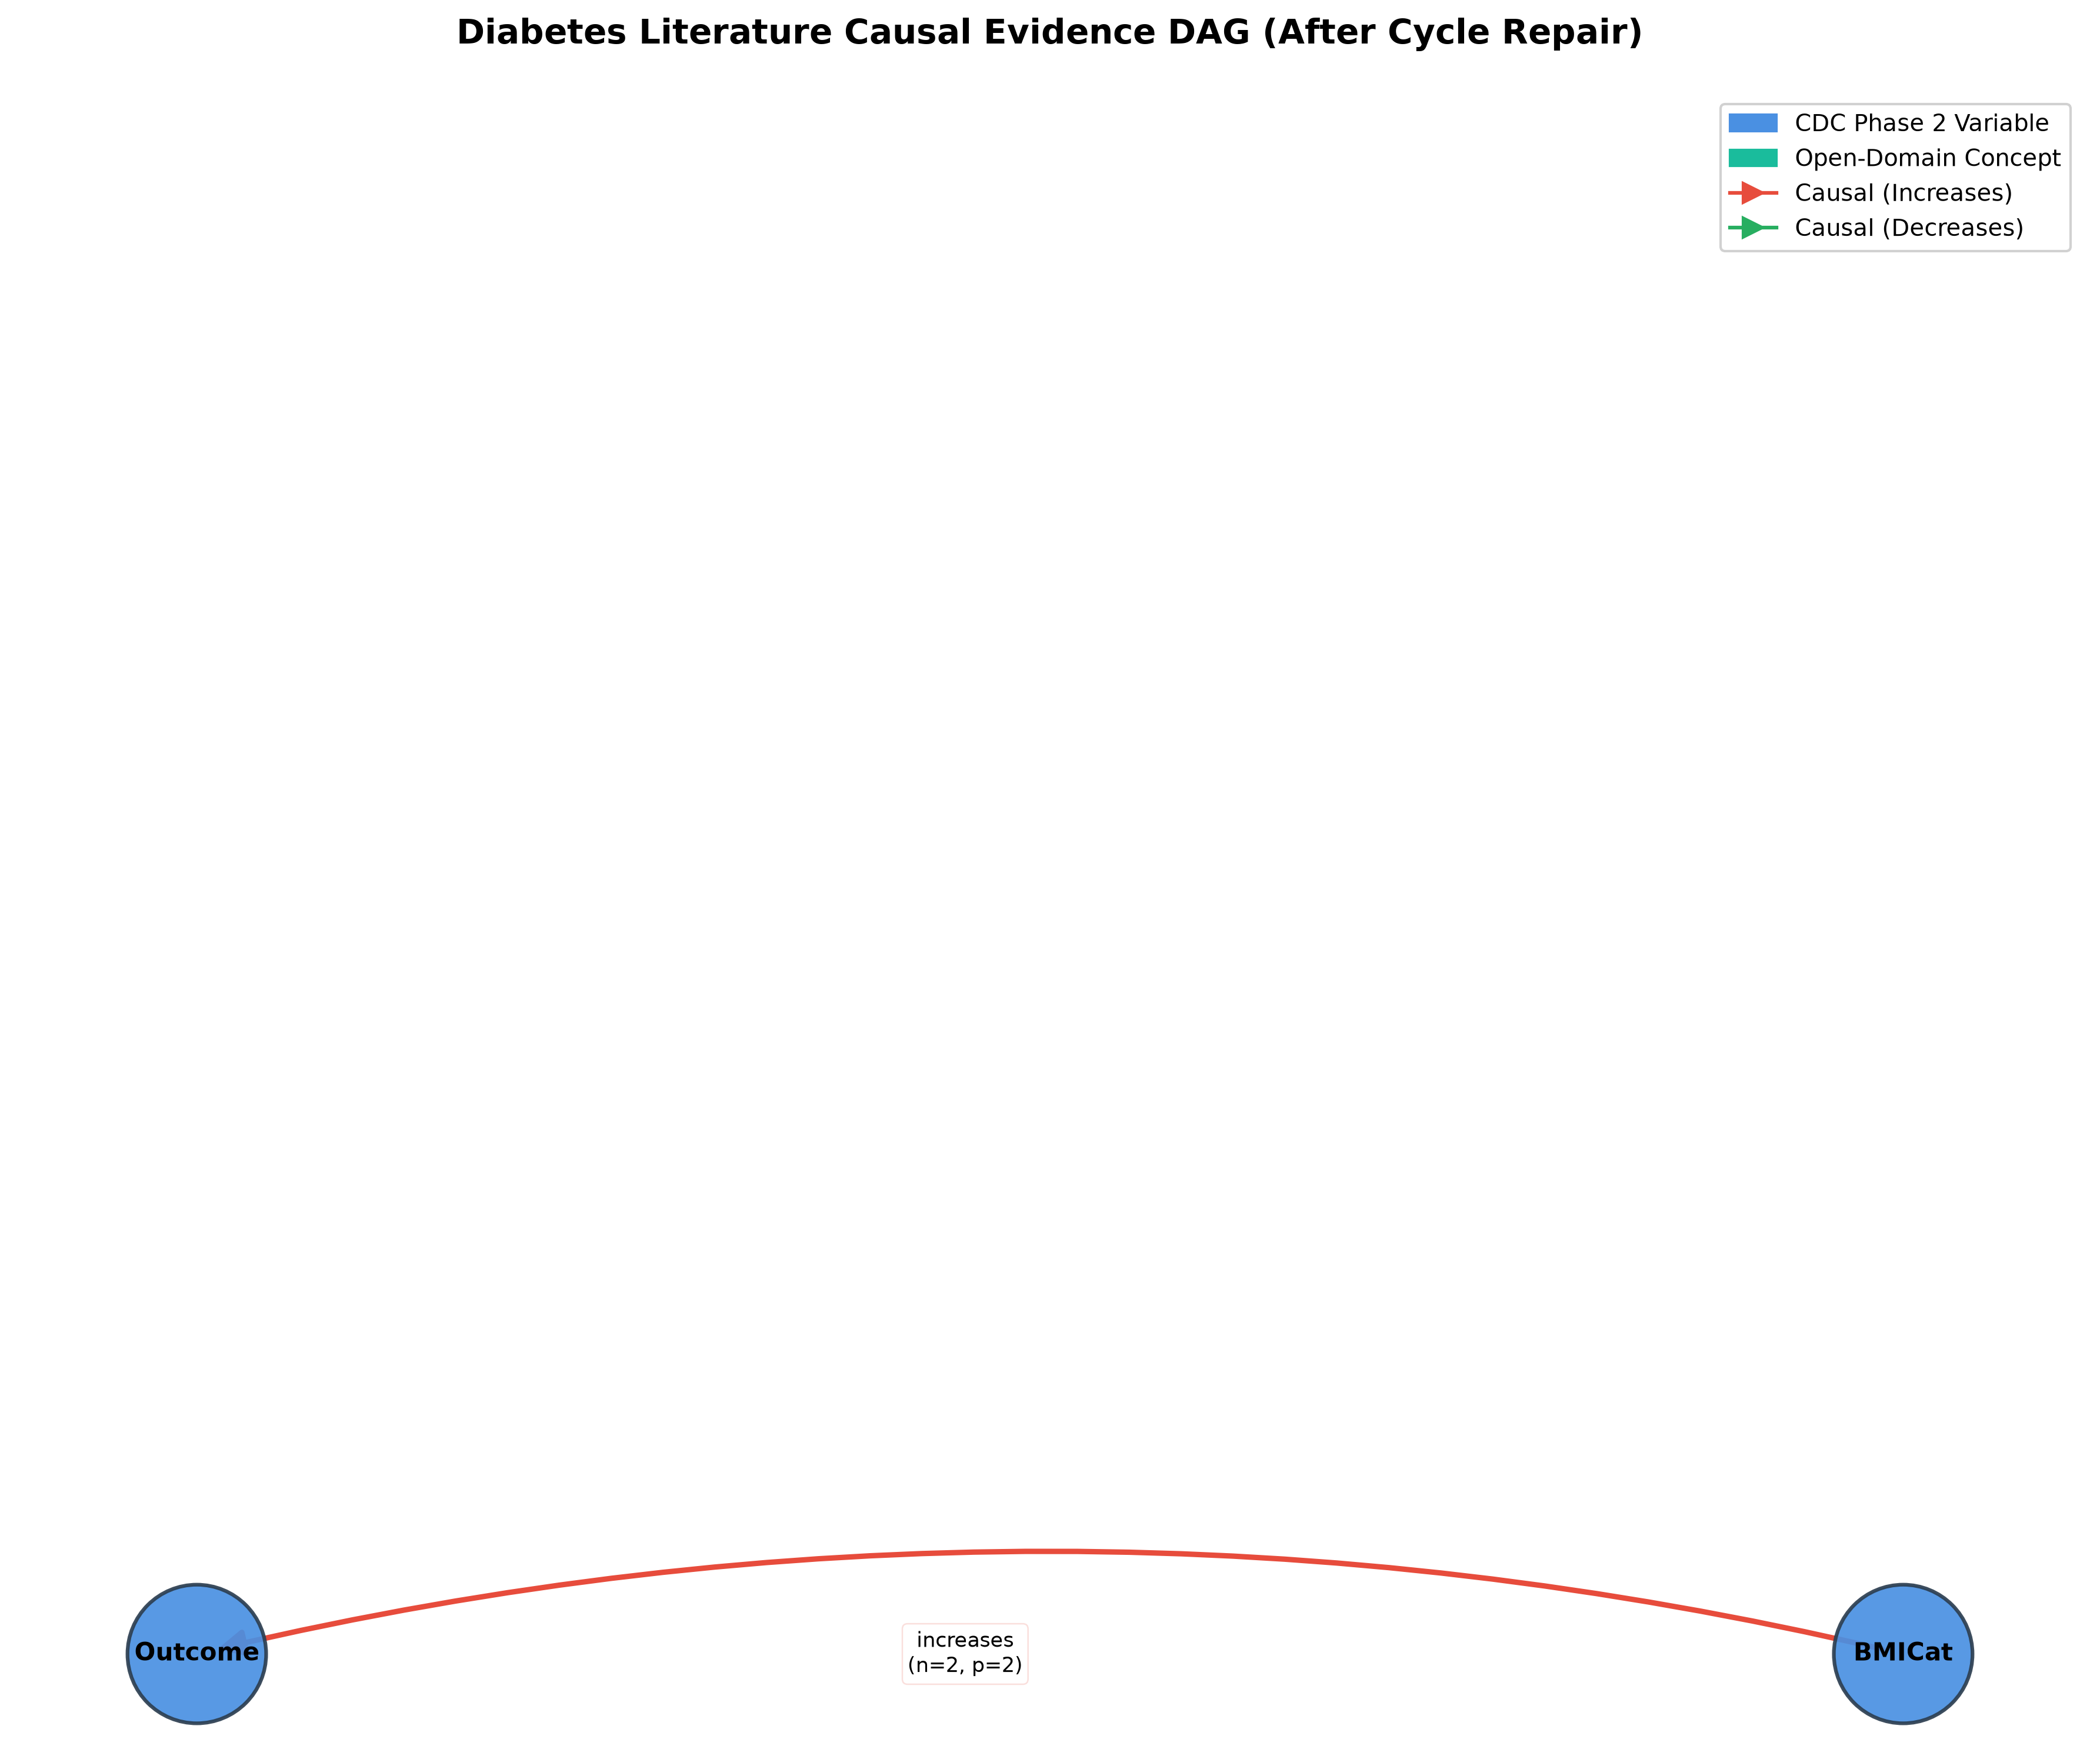
\includegraphics[width=\textwidth]{causal_dag.png}
    \caption{Causal DAG ($\text{BMICat} \rightarrow \text{Outcome}$)}
    \label{fig:causal_dag}
\end{subfigure}
\hfill
\begin{subfigure}[b]{0.52\textwidth}
    \centering
    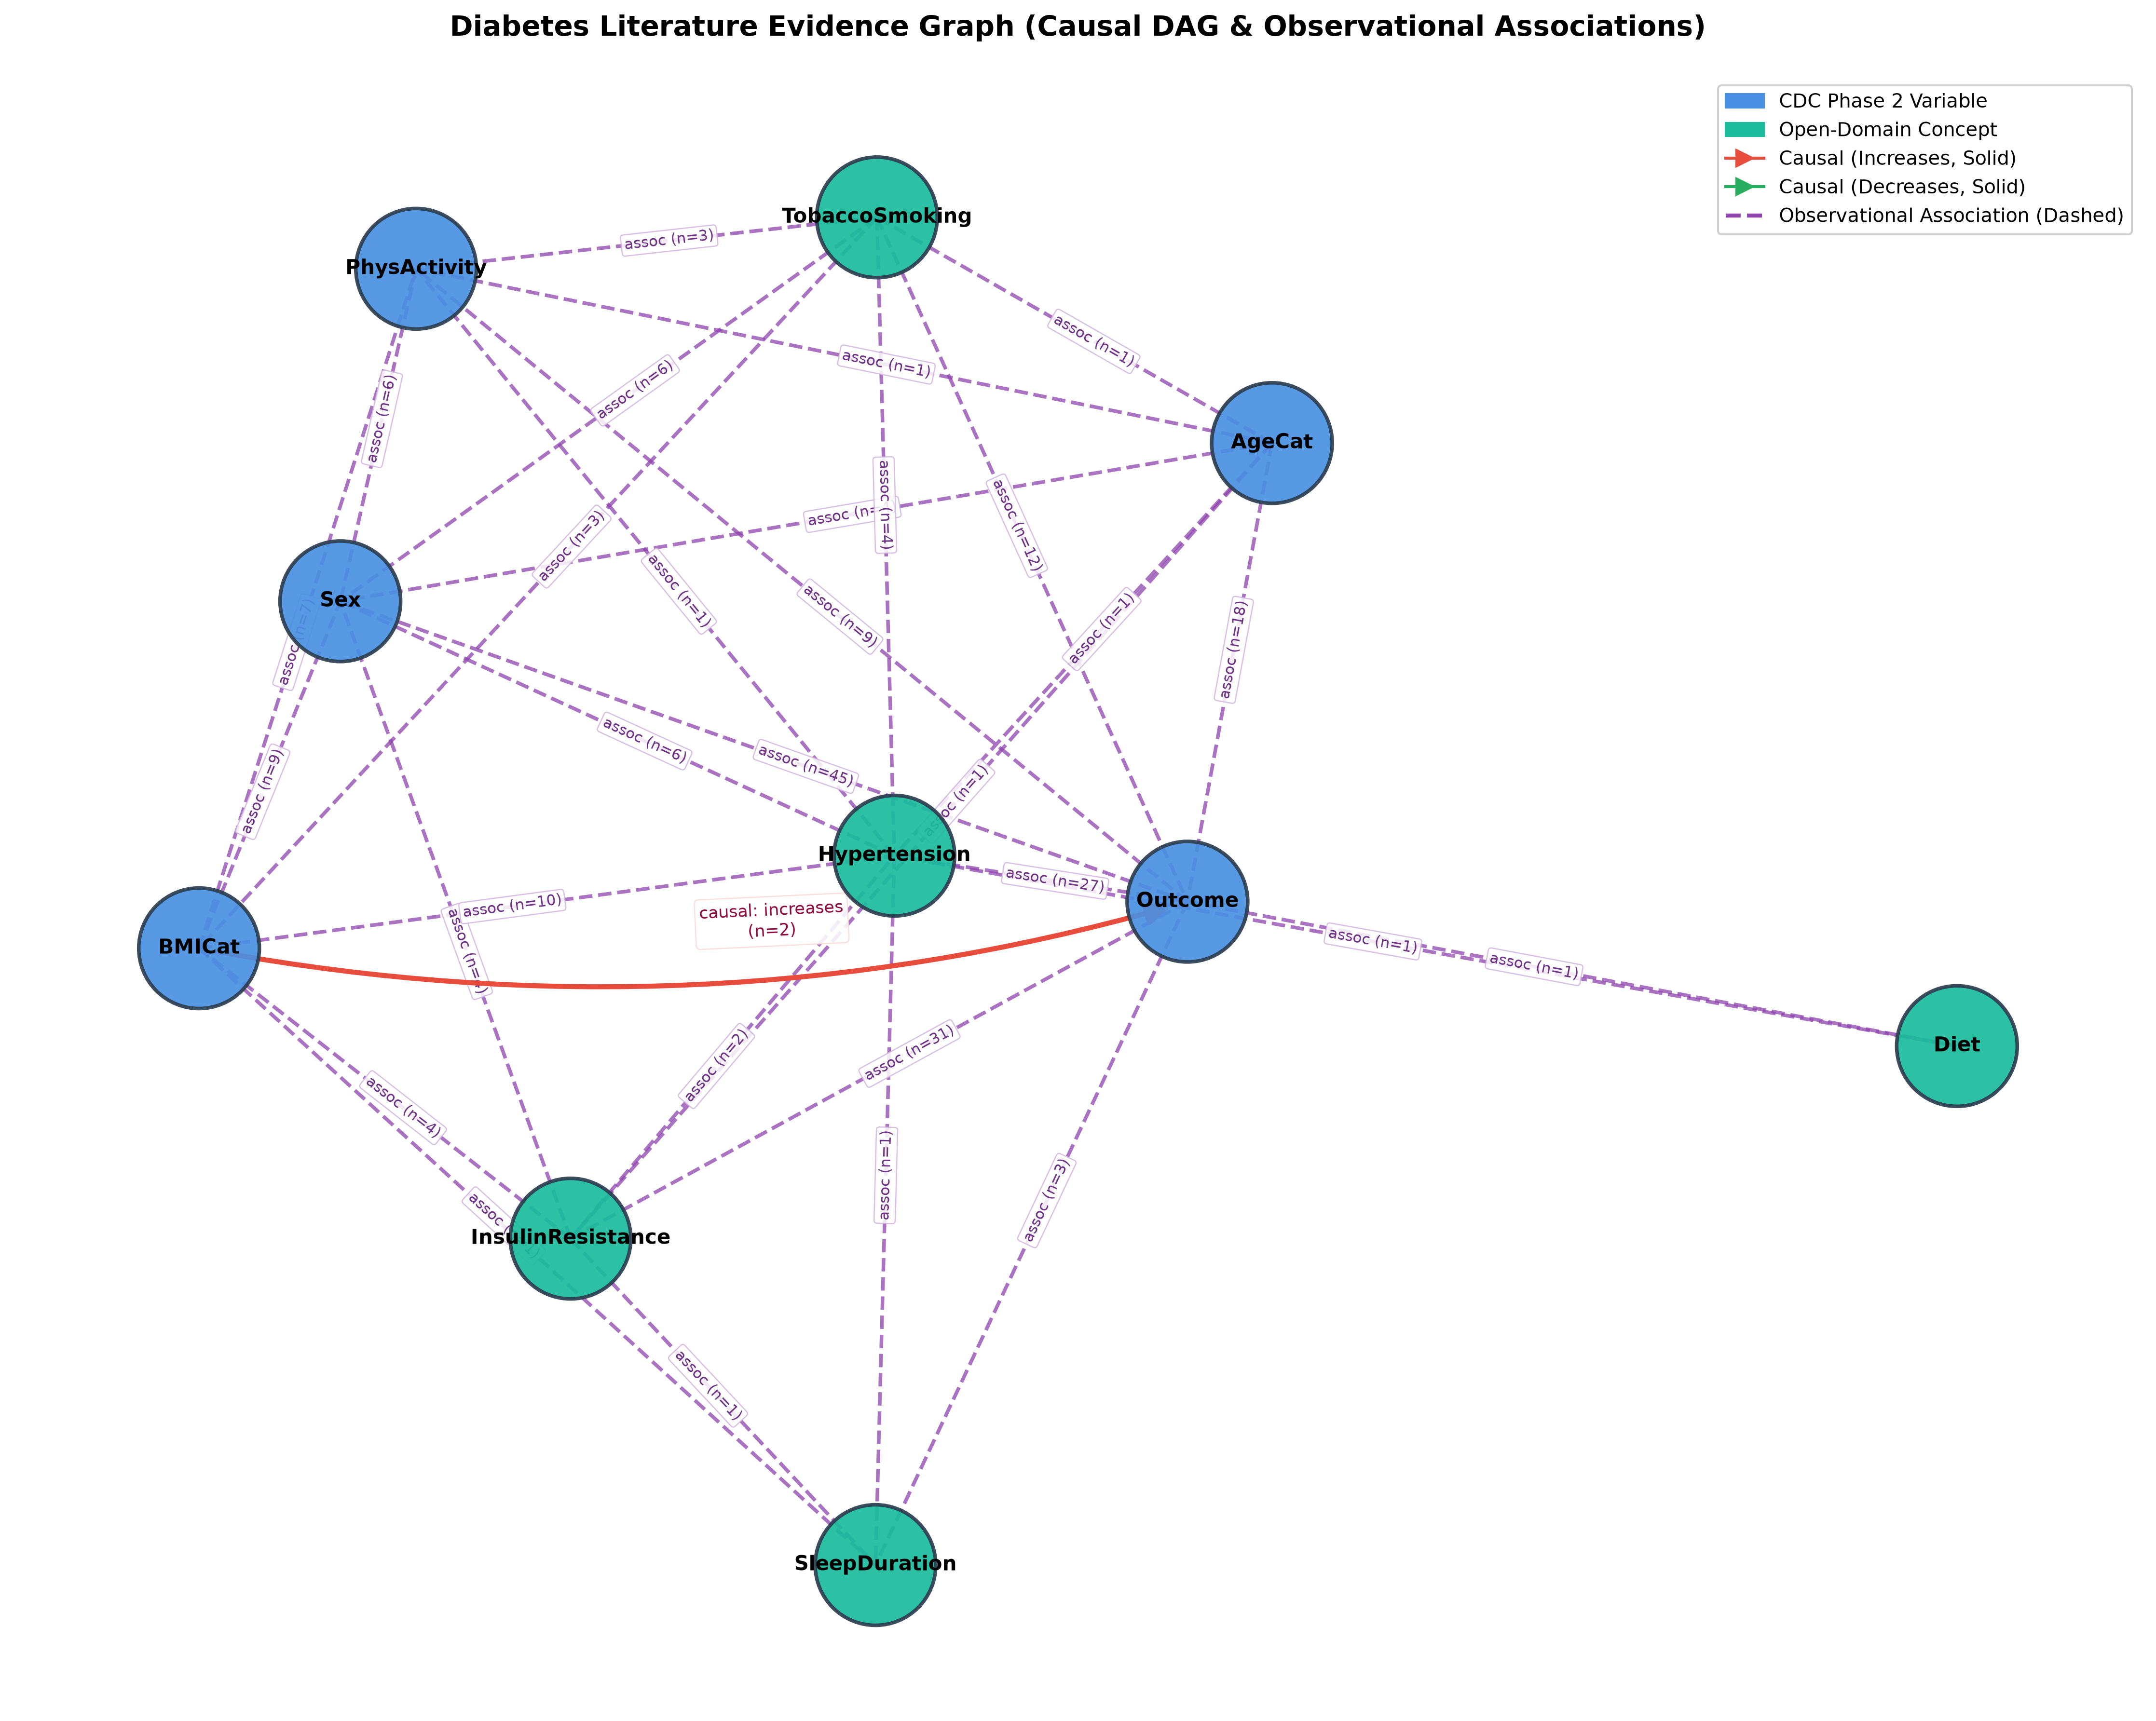
\includegraphics[width=\textwidth]{evidence_graph_after_repair.png}
    \caption{Combined Multi-Relational Evidence Graph}
    \label{fig:combined_graph}
\end{subfigure}
\caption{Visualizations of the reconstructed literature graphs: (a) strictly validated causal DAG; (b) multi-relational network showing solid causal arrows and dashed observational associations.}
\label{fig:evidence_graphs}
\end{figure}

\subsection{Evidence Deduplication and Independence}
In previous versions, duplicate prediction records from identical files inflated edge confidence. We hardened \texttt{\_record\_evidence\_item} to enforce signature deduplication:
\begin{equation}
    \text{Sig} = (\text{extractor\_name}, \text{polarity}, \text{confidence}, \text{reasoning})
\end{equation}
Furthermore, the builder separates three distinct metrics for each edge:
\begin{itemize}[leftmargin=1.5em]
    \item $\text{unique\_evidence\_sentences}$: The count of distinct PubMed sentence identifiers supporting the edge.
    \item $\text{unique\_papers\_count}$: The count of distinct PMIDs citing the claim.
    \item $\text{agreement\_count}$: The number of distinct extraction engines agreeing on the sentence.
\end{itemize}
Multiple extractors agreeing on the same sentence do \textbf{not} artificially increase the scientific literature support count.

\subsection{Deterministic Cycle Repair Algorithm}
To satisfy the DAG contract required by Bayesian Networks, directed causal candidate graphs are monitored for cycles:
\begin{equation}
    \mathcal{C} = \{c \mid c \text{ is a simple cycle in } \mathcal{G}_{\text{causal}}\}
\end{equation}
If $\mathcal{C} \neq \emptyset$, the deterministic heuristic \texttt{IterativeMinConfidenceRemoval} removes the edge minimizing aggregated confidence, breaking ties via minimum citation support count, followed by lexicographical node ordering. In the final validated graph:
\begin{equation}
    |\mathcal{C}| = 0, \quad \text{Removed Edges} = 0, \quad \text{is\_dag} = \text{True}
\end{equation}
The causal DAG is naturally acyclic without requiring edge deletion.

% ==============================================================================
\section{Phase 2 Handoff and Bayesian Network Roadmap}
\label{sec:phase2_handoff}
% ==============================================================================

Phase 2 will integrate the literature evidence graph with individual-level health records from the CDC BRFSS dataset. To prevent scientific overreach, the formal handoff document (\texttt{docs/PHASE\_2\_HANDOFF.md}) defines strict consumption boundaries.

\subsection{Consumable vs. Provisional Artifacts}
\begin{itemize}[leftmargin=1.5em]
    \item \textbf{Approved for Bayesian Network Structure:} $\mathcal{G}_{\text{causal}}$ (\texttt{evidence\_graph\_after\_repair.graphml}), providing the structural prior $\text{BMICat} \rightarrow \text{Outcome}$.
    \item \textbf{Approved for Latent Confounding Exploration:} $\mathcal{G}_{\text{assoc}}$ (\texttt{association\_graph.graphml}), providing 31 observational associations.
    \item \textbf{Restricted:} \texttt{sample.jsonl} must \textbf{not} be cited as human ground truth in Phase~2 publications until dual clinical review is executed.
\end{itemize}

\subsection{Mandatory Epidemiological Assumptions}
When fitting Conditional Probability Distributions (CPDs) $P(Y \mid \text{Parents}(Y))$ on CDC survey microdata, Phase~2 must explicitly declare:
\begin{enumerate}[leftmargin=1.5em]
    \item \textbf{Causal Sufficiency:} Assumes no unmeasured confounders simultaneously determine exposure and outcome—an assumption known to be violated in observational survey data.
    \item \textbf{Observational vs. Interventional Discrepancy:}
    \begin{equation}
        P(\text{Outcome}=1 \mid \text{BMICat}=\text{obese}) \neq P(\text{Outcome}=1 \mid do(\text{BMICat}=\text{obese}))
    \end{equation}
    Phase~2 can computationally simulate $do$-interventions under explicitly stated DAG assumptions, but observational data alone cannot substitute for randomized controlled clinical trials (RCTs).
\end{enumerate}

% ==============================================================================
\section{Technical Verification and Acceptance Audit}
\label{sec:verification}
% ==============================================================================

All 23 acceptance criteria specified in the master audit plan were verified. Table~\ref{tab:acceptance_summary} summarizes the audit status across core dimensions.

\begin{table}[htbp]
\centering
\small
\caption{Summary of final acceptance checklist (\texttt{results/final\_audit/final\_acceptance\_checklist.json}).}
\label{tab:acceptance_summary}
\begin{tabularx}{\textwidth}{l c X}
\toprule
\textbf{Acceptance Criterion} & \textbf{Status} & \textbf{Audit Verification Evidence} \\
\midrule
Pre-repair backup preserved & \textbf{PASS} & Saved in \texttt{backups/audit\_pre\_repair\_20261025/}; excluded by \texttt{.gitignore}. \\
Annotation provenance truthful & \textbf{PASS} & All 250 records marked \texttt{PROVISIONAL\_RULE\_PSEUDO\_GOLD}, \texttt{human\_reviewed: false}. \\
Synthetic agreement disclaimed & \textbf{PASS} & Reclassified as \texttt{SYNTHETIC\_PIPELINE\_CONSISTENCY\_CHECK}; human queue created. \\
DistilBERT alias retracted & \textbf{PASS} & Documented as \texttt{KeywordHeuristic} baseline; duplicate files excluded. \\
Causal filters hardened & \textbf{PASS} & Excluded dementia risk (\texttt{42828458}) and mediator (\texttt{42901975}); verified \texttt{BMICat->Outcome}. \\
Evaluation metrics hardened & \textbf{PASS} & Detects duplicate IDs; penalizes missing predictions; flags zero-support test causal class. \\
Offline reconstruction verified & \textbf{PASS} & \texttt{./run.sh --from-saved-predictions} runs in 3.8s with 0 API/network calls. \\
Full test suite passes & \textbf{PASS} & \texttt{./run.sh test} passes all 68 unit and regression tests in 5.47s. \\
Phase 2 handoff established & \textbf{PASS} & \texttt{docs/PHASE\_2\_HANDOFF.md} defines structural usage and observational caveats. \\
\bottomrule
\end{tabularx}
\end{table}

% ==============================================================================
\section{Conclusion and Future Work}
\label{sec:conclusion}
% ==============================================================================

Phase~1 of the \textit{Neuro-Symbolic Causal Inference for Diabetes-Related Health Evidence} project has reached a verified, reproducible, and offline-capable baseline. By systematically eliminating misleading provenance claims, separating heuristic baselines from neural models, hardening epidemiological causal filters, and disclosing class-imbalance boundaries on held-out data, the project establishes a scientifically defensible foundation. 

Immediate next steps prior to academic peer review include: (1) executing dual-blind human adjudication across the 50-pair review queue in \texttt{data/annotations/human\_annotation\_queue.jsonl}; (2) enriching the held-out test split with verified causal examples to enable empirical causal generalization measurement; and (3) initializing Phase~2 Bayesian Network structure learning with the verified causal DAG skeleton.

% ==============================================================================
\bibliographystyle{plain}
\bibliography{references}
% ==============================================================================

\end{document}
